\documentclass{article}

%%%%%%%%%%%%%%%%%%%%%%%%%%%%%%%%%%%%%%%%

\usepackage[utf8]{inputenc}

%%%%%%%%%%%%%%%%%%%%%%%%%%%%%%%%%%%%%%%%

\usepackage[dvipsnames]{xcolor} %may result in an error if you are using beamer with tikz. To go around it, include usenames and dvipsnames options when defining the document class, e.g. \documentclass[usenames,dvipsnames]{beamer}
\usepackage{tikz}
\usepackage{pgfplots}
\pgfplotsset{compat=1.5}

%\usetikzlibrary{external}
%\tikzexternalize
%\tikzsetexternalprefix{tikzexternal/}

%%%%%%%%%%%%%%%%%%%%%%%%%%%%%%%%%%%%%%%%

\usepackage{amsmath,amsfonts,amssymb}
\renewcommand{\baselinestretch}{1.0}
\usepackage{graphicx}
\usepackage[colorlinks=true, allcolors=blue]{hyperref}
\usepackage{color, colortbl}
\usepackage{lscape}
\usepackage{enumitem}
%\usepackage{chngcntr}
%\counterwithin{figure}{section}
%\counterwithin{table}{section}
\usepackage{booktabs,caption}
\usepackage[flushleft]{threeparttable}

%%%%%%%%%%%%%%%%%%%%%%%%%%%%%%%%%%%%%%%%

\setlength{\parindent}{0pt}
\setlength{\parskip}{\medskipamount}

%%%%%%%%%%%%%%%%%%%%%%%%%%%%%%%%%%%%%%%%

\usepackage{newtxtext,newtxmath}

% Instead of the above, use this for arXiv:

%\usepackage{txfonts}
%\usepackage{textcomp}
%\usepackage{eurosym}
%\let\texteuro\euro

%%%%%%%%%%%%%%%%%%%%%%%%%%%%%%%%%%%%%%%%

\newcommand{\unit}[1]{\ensuremath{\mathrm{#1}}}
\newcommand{\micron}{\mbox{\textmu m}}
\renewcommand{\deg}{\mbox{deg}}
\newcommand{\sqdeg}{\mbox{$\deg^2$}}
\newcommand{\persqdeg}{\mbox{$\deg^{-2}$}}
\newcommand{\arcmin}{\mbox{arcmin}}
\newcommand{\sqarcmin}{\mbox{\arcmin$^2$}}
\newcommand{\persqarcmin}{\mbox{\arcmin$^{-2}$}}
\newcommand{\arcsec}{\mbox{arcsec}}
\newcommand{\sqarcsec}{\mbox{\arcsec$^2$}}
\newcommand{\persqarcsec}{\mbox{\arcsec$^{-2}$}}
\newcommand{\sqmm}{\mbox{mm$^2$}}
\newcommand{\deighty}{\ensuremath{d_{80}}}
\newcommand{\Hs}{\mbox{$H_\mathrm{s}$}}
\newcommand{\Ravg}{\mbox{$R_\mathrm{avg}$}}
\newcommand{\Tavg}{\mbox{$T_\mathrm{avg}$}}
\newcommand{\mm}{\mbox{mm}}

\newcommand{\code}[1]{{\ttfamily #1}}

%%%%%%%%%%%%%%%%%%%%%%%%%%%%%%%%%%%%%%%%

\begin{document}

\pagestyle{empty}

\begin{center}

{\Large \bfseries DDRAGUITO: Detector and Filter Wheel Laboratory Verification}

\vspace{2cm}

\begin{tabular}{ll}
Prepared by:&Alan M. Watson\\
Reviewed by:&\\
Approved by:&\\
%DDRAGO Reference:&Document 2\\
COLIBRÍ Reference:&COLIBRI-UNAM-???\\
Version:&0.0\\
Date:&12 November 2020\\
\end{tabular}

\vspace{\fill}

COLIBRÍ Project\\
Instituto de Astronom{\'\i}a\\
Universidad Nacional Aut\'onoma de M\'exico

\end{center}

\newpage

\clearpage
\section*{Version History}

\begin{itemize}

\item Version 1.0 of 12 November 2020

\begin{itemize}
    \item Initial version.
\end{itemize}

\end{itemize}

%%%%%%%%%%%%%%%%%%%%%%%%%%%%%%%%%%%%%%%%%

\clearpage
%%%%%%%%%%%%%%%%%%%%%%%%%%%%%%%%%%%%%%%%%

\pagestyle{plain}

\setcounter{tocdepth}{2}
\tableofcontents
\newpage

%\listoffigures
%\newpage

%\listoftables
%\newpage

%%%%%%%%%%%%%%%%%%%%%%%%%%%%%%%%%%%%%%%%%

\section{Introduction}

The DDRAGUITO detector is a Teledyne e2v CCD231-84-1-E90. This is a grade-1 device with deep-depletion and "astro multi-2" anti-reflection coating, but without fringe suppression. The detector is packaged in a Spectral Instruments 1100-series head and is cooled by a Brookes Polycold PCC Compact Cooler with PT-30 gas. The power supply and cryogen compressor are in a separate service cabinet. The detector is read using Spectral Instrument's SI Image software running on a Windows PC. The TCS server communicates with this software using its TCP/IP interface. 

\section{Detector Format}

\begin{figure}
\begin{center}
\begin{tikzpicture}[scale=24]
\draw (-0.2098,-0.2056) -- (+0.2098,-0.2056) -- (+0.2098,+0.2056) -- (-0.2098,+0.2056) -- cycle;
\draw (-0.2048,-0.2056) -- (+0.2048,-0.2056) -- (+0.2048,+0.2056) -- (-0.2048,+0.2056) -- cycle;
\draw [dotted] (-0.2098,0) -- (+0.2098,0);
\draw [dotted] (0,-0.2056) -- (0,+0.2056);
\draw[->] (-0.025,-0.025) -- (-0.025,-0.175) -- (-0.175,-0.175);
\draw[->] (+0.025,-0.025) -- (+0.025,-0.175) -- (+0.175,-0.175);
\draw[->] (-0.025,+0.025) -- (-0.025,+0.175) -- (-0.175,+0.175);
\draw[->] (+0.025,+0.025) -- (+0.025,+0.175) -- (+0.175,+0.175);
\draw (-0.12,-0.12) node {0};
\draw (+0.12,-0.12) node {1};
\draw (-0.12,+0.12) node {2};
\draw (+0.12,+0.12) node {3};
\draw[->] (-0.2,-0.25) -- (+0.2,-0.25) node [anchor=west] {$x$};
\draw[->] (-0.25,-0.2) -- (-0.25,+0.2) node [anchor=south] {$y$};
\draw[dashed] (-0.2096,-0.2048) -- (-0.2096,+0.2048) -- (+0.2096,+0.2048) -- (+0.2096,-0.2048) -- cycle; 
\draw[dashed] (-0.1024,-0.1024) -- (-0.1024,+0.1024) -- (+0.1024,+0.1024) -- (+0.1024,-0.1024) -- cycle; 
\draw[dashed] (-0.0512,-0.0512) -- (-0.0512,+0.0512) -- (+0.0512,+0.0512) -- (+0.0512,-0.0512) -- cycle; 
\end{tikzpicture}
\caption{The format of the CCD. The full format is an active area is $4096~\mbox{columns} \times 4112~\mbox{rows}$ and with 50 columns of underscan at the start and end of each row, giving a total format of $4196~\mbox{columns} \times 4112~\mbox{rows}$. It is read in four quadrants, as shown by the dashed line and the arrows. The parallel clocks move charge vertically and the serial clocks move charge horizontally. The quadrants are numbered 0 to 3 as shown. The dashed lines show the \code{4kx4k}, \code{2kx2k}, and \code{1kx1k} windows.}
\label{figure:format}
\end{center}
\end{figure}

The detector has a active area of  $4096~\mbox{columns} \times 4112~\mbox{rows}$. It is read using the “split full frame read-out through four amplifiers” scheme described on page 17 of the Teledyne e2v data sheet. The controller adds 50 columns of underscan at the start and end of each row, giving a total size of $4196~\mbox{columns} \times 4112~\mbox{rows}$. This is show in Figure~\ref{figure:format}

The SI Image software allows us to define windows provided they are centered on the detector. We define three windows that we expect will be useful for science, named \code{4kx4k}, \code{2kx2k}, and \code{1kx1k}, described below and shown in Figure~\ref{figure:format}. Each window can be used with a binning of 1, 2, or 4 pixels (both vertically and horizontally).

The \code{4kx4k} window has an active area of $4096~\mbox{columns} \times 4096~\mbox{rows}$, centered on the detector, with 48 columns of underscan at the start and end of each row, giving a total size of $4192~\mbox{columns} \times 4096~\mbox{rows}$.

The \code{2kx2k} window has an active area of $2048~\mbox{columns} \times 2048~\mbox{rows}$, centered on the detector, without underscan.

The \code{1kx1k} window has an active area of $1024~\mbox{columns} \times 1024~\mbox{rows}$, centered on the detector, without underscan.

We do not typically use the full native format. The first and last rows show unusual behavior (higher values in the underscan regions and lower values in the active regions). Also, the underscans of 50 columns are not commensurate with a binning of 4.  However, the full native format is available as an engineering mode with window name \verb|full|.

\section{Detector Read Modes}

The controller offers three read frequencies (1.01~MHz, 502.5~kHz, and 332.2~kHz) and two gain modes (low and high). These are exposed as “read modes”, which are summarized in Table~\ref{table:read-modes}.

\begin{table}[]
\begin{center}
\begin{tabular}{ccc}
\hline
Read Mode&Frequency&Gain\\
\hline
\code{0}&1.01~MHz&low\\
\code{1}&1.01~MHz&high\\
\code{2}&502.5~kHz&low\\
\code{3}&502.5~kHz&high\\
\code{4}&332.2~kHz&low\\
\code{5}&332.2~kHz&high\\
\hline
\end{tabular}
\end{center}
    \caption{Read Modes}
    \label{table:read-modes}
\end{table}

\section{Detector Overhead}

\begin{table}
\caption{Overheads}
\label{table:overheads}
\begin{center}
\begin{tabular}{cccc}
\hline
Window&\multicolumn{3}{c}{Binning}\\
&1&2&4\\
\hline
\code{4kx4k}&7.0&3.5&2.4\\
\code{2kx2k}&5.1&3.9&3.4\\
\code{1kx1k}&4.7&4.1&4.0\\
\hline
\end{tabular}
\end{center}
\end{table}

The controller offers read frequencies of 1.01~MHz, 502.5~kHz, and 332.2~kHz. The only frequency offered for science use is 1.01~MHz (read modes \code{0} and \code{1}). The other frequencies are available in engineering modes.

The exposure overhead was measured by taking three bias images in each configuration (window and binning) and determining the median time between the exposure being commanded in TCS and the TCS forking a process to write the image. Thus, it includes both pre-exposure overhead (e.g., communicating with the controller and resetting the detector) and post-exposure overhead (e.g., reading the detector and transfering the pixel data from the Windows PC to the TCS Linux PC), but does not include any overhead for writing the image to a FITS file as this is effectively parallelized by the TCS. The results are shown in Table~\ref{table:overheads}.

One might naively expect the overhead for the \code{4kx4k} window with binning 1 to be about 4.2 seconds (for $2098 \times 2048$ pixels read at 1.01~MHz). However, investigation shows that the pre-exposure delay is about 0.5 seconds, the actual read time from the detector to the Windows PC is about 5.9 seconds, and the transfer time from the Windows PC to the Linux PC is about 0.6 seconds.

The overheads for the \code{4kx4k} window with binning are more or less as expected under the assumption that the parallel transfer is faster by a factor equal to the binning but the serial transfer remains the same speed.

On the other hand, the overheads for the other windows are somewhat puzzling. One might expect the overhead for the \code{2kx2k} window with binning 1 to be similar to that for the \code{4kx4k} window with a binning of 2 (since one might assume that in each quadrant there are about 1k parallel transfers without serial transfers and 1k parallel transfers with serial transfers), but this is not the case; the overhead for the \code{2kx2k} window with binning 1 is 5.1 seconds whereas that for the \code{4kx4k} window with a binning of 2 is 3.5 seconds.

Even more puzzling, the overhead for the binned CCD is \emph{larger} for the smaller windows. For example, with binning 2, the \code{4kx4k} window has an overhead of 3.5 seconds, the \code{2kx2k} window has an overhead of 3.9 seconds, and the \code{1kx1k} window has an overhead of 4.1 seconds.

We have only limited experience with the other read frequencies. The overhead for the \code{4kx4k} window with binning 1 is 11.6 seconds at 502.5kHz and 15.8 seconds at 332.2~kHz.

The relevant requirement GFT-REQ-163 is that the overhead (actually, “read-out time” but the overhead is more appropriate) for the detectors shall be less than 5 seconds. We do not meet this requirement, since the overhead for the \code{4kx4k} window with binning 1 is 7.0 seconds. Since our ability to improve this situation is limited, together with the project we have decided to accept this non-conformity. For exposures of 60 seconds, it effectively reduces the efficiency of the instrument by a factor of $(60+5)/(60+7) \approx 0.97$.

\section{Illumination System}

\begin{figure}
\begin{center}
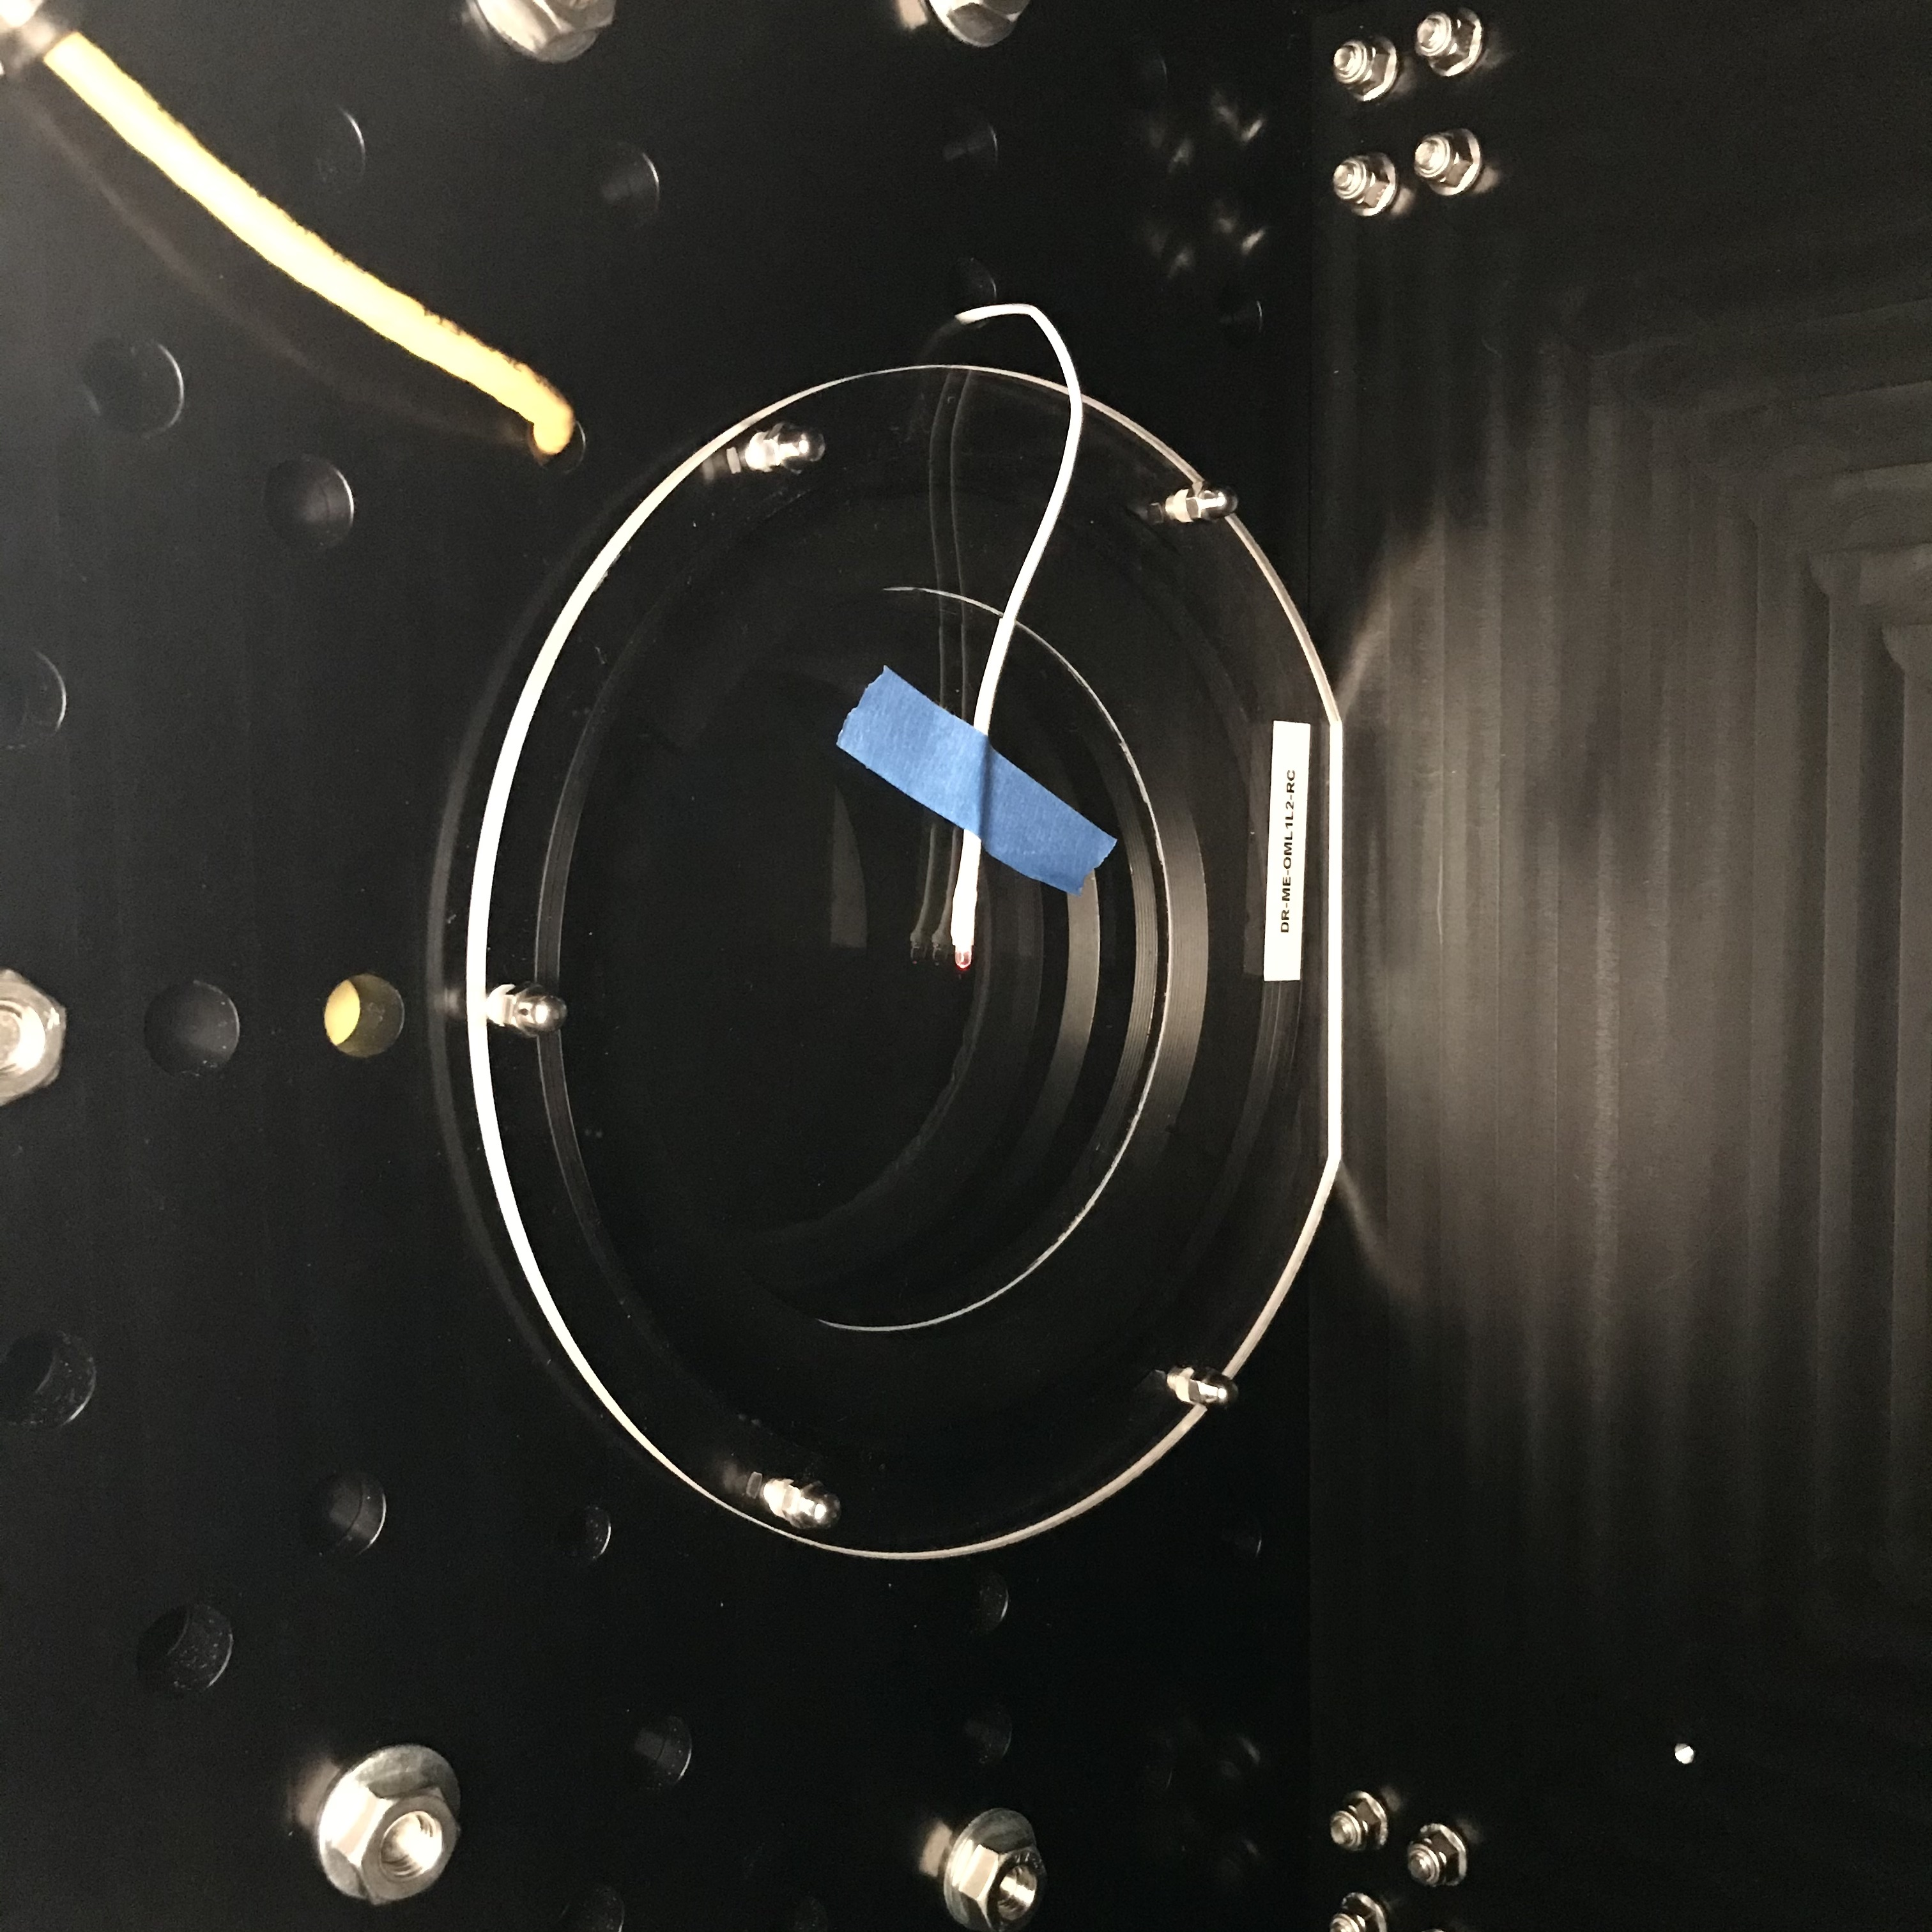
\includegraphics[width=0.45\linewidth]{IMG_1296.jpg}
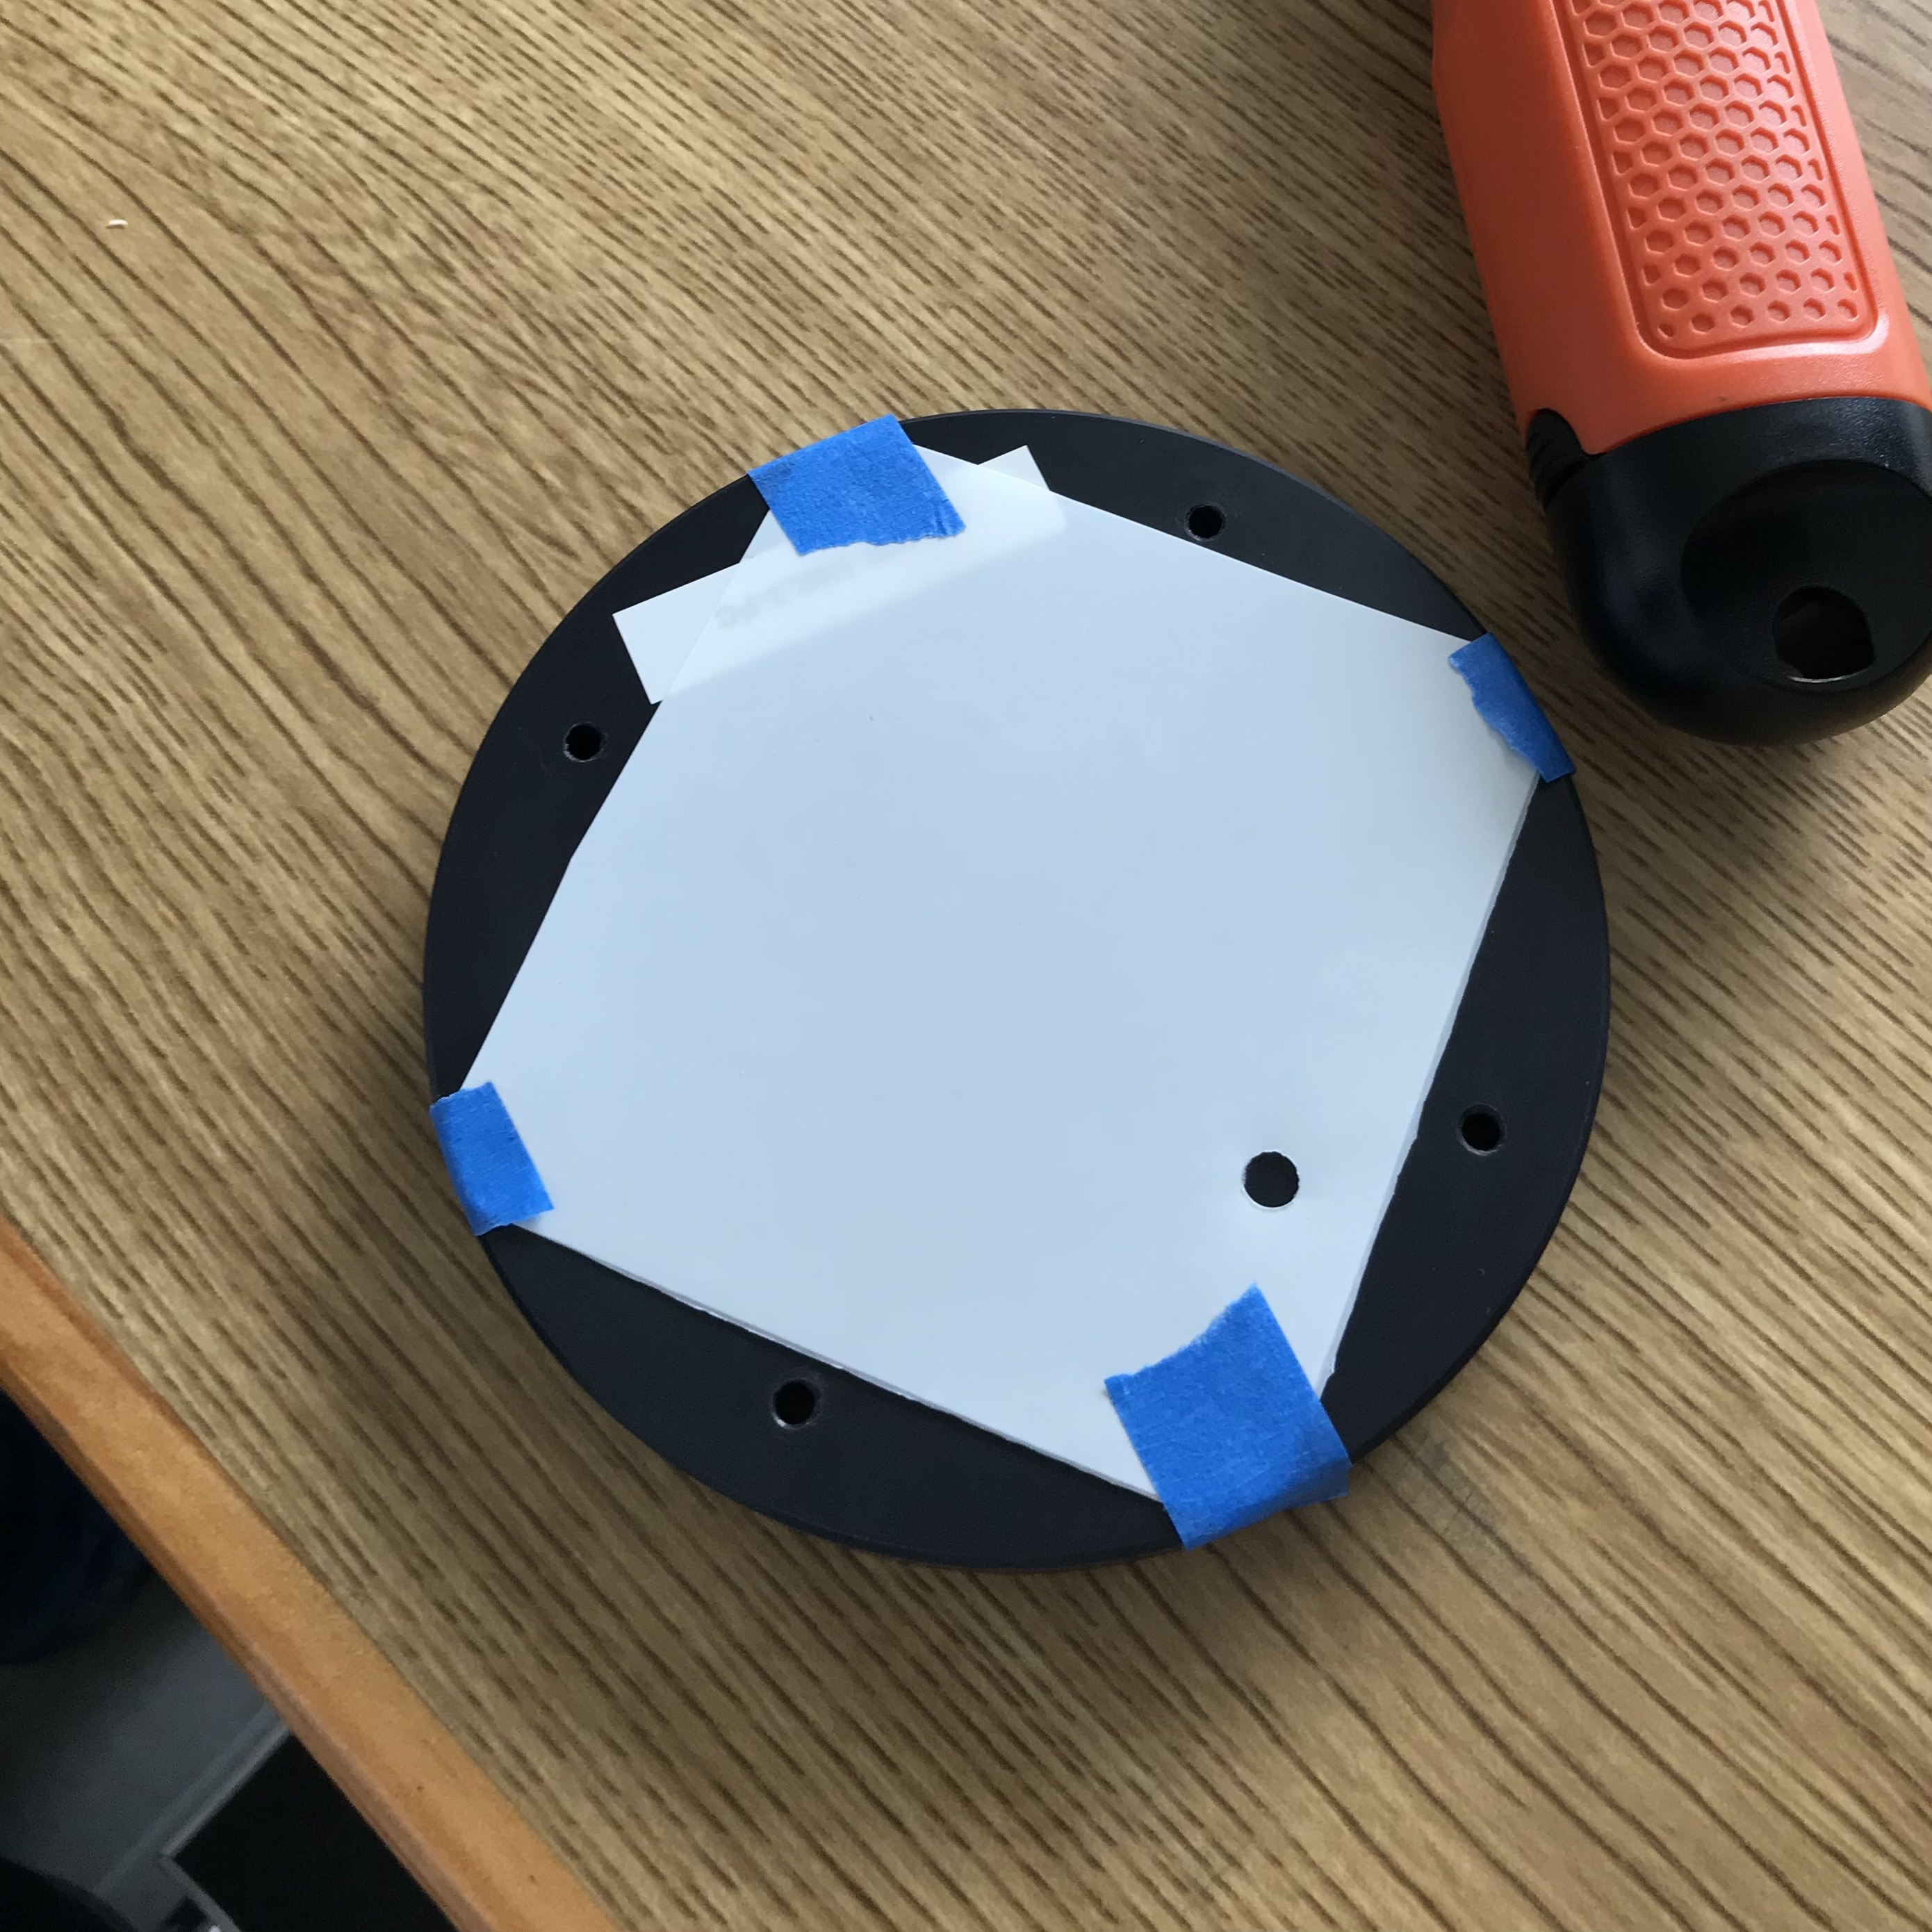
\includegraphics[width=0.45\linewidth]{IMG_1301.jpg}
\end{center}
\caption{The illumination system for the laboratory tests consisted of a stablized LED in the middle of the rear cover of the L1L2 barrel (left) and a white plastic difuser on the front cover of the L3 front cover (right).}
\label{figure:illumination-system}
\end{figure}

For tests that require illumination, we installed a LED supplied by a stabilized power supply approximately at the center of the rear cover of the L1L2 barrel (DR-ME-OML1L2-RC). The power supply was connected to one of the iBoot-PDUs to allow us to automate the tests. The bare LED cast sharp shadows from the damage to the first surface of L3 on the detector. Therefore, we installed a sheet of white plastic on the front cover of the L3 barrel (DR-ME-OML3-FC) to act as a difuser. The system is shown in Figure~\ref{figure:illumination-system}. The level of the LED was adjusted to give about 1000 DN/s/px in readmode 0.

The final illumination pattern appears to be quite uniform, but the solid angle of the illumination at each point in the detector will be much larger than for an astronomical source imaged through on the telescope. This will, for example, modify the shutter exposure-time correction.

\section{Detector Bias Level, Read Noise, and Gain}

We determined the bias level, read noise, and gain in each detector quadrant for both supported science read modes (0 and 1), all three supported science windows (\code{4kx4k}, \code{2kx2k}, \code{1kx1k}), and all three supported science binnings (1, 2, and 4).

For each configuration, we took two biases (with the LED switched off) and two flats (with the LED switched on). The exposure time was 16 seconds for binning 1, 4 seconds for binning 2, and 1 second for binning 4, which gave approximately the same charge per pixel in each case (about 16k DN for read mode 0 and 32k DN for read mode 1).

The noise per pixel at high signal $n$ in electrons is $\sigma_n = \sqrt{n}$. Thus, with a gain of $g$, the noise per pixel at high signal $N=n/g$ in DN is $\sigma_N = (\sqrt{Ng})/g = \sqrt{N/g}$ in DN. Thus, the gain $g$ is given by $N/\sigma_N^2$. The value of $\sigma_N$ is estimated by the standard deviation in the difference between the two flats divided by $\sqrt{2}$. The value of $N$ is estimated by the mean in the flats after subtracting a bias.

The noise per pixel in the biases in electrons is just the read-noise $r_n$. Thus, with a gain of $g$, the noise per pixel in the biases in DN is $r_N = r_n/g$. The value of $r_N$ is estimated by the standard deviation in the difference between the two flats divided by $\sqrt{2}$. The value of $r_n$ is estimated by $gr_N$.

\begin{table}
\begin{center}\footnotesize
    \begin{tabular}{cccccccc}
    \hline
Read Mode&Window&Binning&Quadrant&Bias Level&Gain&Read Noise&Read Noise\\
&&&&(DN)&(e/DN)&(DN)&(e)\\
\hline
0&\code{4kx4k}&1
  &0& 510.06& 2.22& 2.97& 6.6\\
&&&1& 509.99& 2.23& 3.05& 6.8\\
&&&2& 509.57& 2.23& 2.90& 6.5\\
&&&3& 509.91& 2.23& 2.95& 6.6\\
0&\code{4kx4k}&2
  &0& 502.18& 2.16& 2.98& 6.4\\
&&&1& 494.55& 2.19& 3.09& 6.8\\
&&&2& 493.34& 2.17& 2.91& 6.3\\
&&&3& 504.71& 2.19& 3.01& 6.6\\
0&\code{4kx4k}&4
  &0& 502.16& 2.15& 3.01& 6.5\\
&&&1& 497.14& 2.16& 3.08& 6.7\\
&&&2& 497.72& 2.16& 2.95& 6.4\\
&&&3& 503.50& 2.16& 3.03& 6.5\\
\hline
0&\code{2kx2k}&1
  &0& 504.32& 2.24& 2.98& 6.7\\
&&&1& 504.18& 2.25& 3.11& 7.0\\
&&&2& 503.31& 2.27& 2.94& 6.7\\
&&&3& 504.18& 2.26& 2.98& 6.7\\
0&\code{2kx2k}&2
  &0& 498.09& 2.15& 2.98& 6.4\\
&&&1& 495.77& 2.17& 3.12& 6.8\\
&&&2& 495.43& 2.20& 2.90& 6.4\\
&&&3& 500.47& 2.14& 3.00& 6.4\\
0&\code{2kx2k}&4
  &0& 501.89& 2.15& 2.99& 6.4\\
&&&1& 497.43& 2.07& 3.12& 6.4\\
&&&2& 498.21& 2.15& 2.92& 6.3\\
&&&3& 503.44& 2.10& 3.03& 6.4\\
\hline
0&\code{1kx1k}&1
  &0& 500.02& 2.25& 2.99& 6.7\\
&&&1& 500.02& 2.26& 3.13& 7.1\\
&&&2& 498.94& 2.24& 2.97& 6.7\\
&&&3& 499.91& 2.25& 2.98& 6.7\\
0&\code{1kx1k}&2
  &0& 498.51& 2.15& 3.00& 6.5\\
&&&1& 495.83& 2.20& 3.14& 6.9\\
&&&2& 495.34& 2.21& 2.93& 6.5\\
&&&3& 500.39& 2.20& 3.00& 6.6\\
0&\code{1kx1k}&4
  &0& 501.99& 2.16& 3.00& 6.5\\
&&&1& 497.55& 2.19& 3.14& 6.9\\
&&&2& 498.34& 2.15& 2.91& 6.3\\
&&&3& 503.43& 2.15& 3.03& 6.5\\
\hline
\end{tabular}
\end{center}
\caption{Read Parameters for Read Mode 0}
\label{table:read-parameters-0}
\end{table}

\begin{table}
\begin{center}\footnotesize
    \begin{tabular}{cccccccc}
    \hline
Read Mode&Window&Binning&Quadrant&Bias Level&Gain&Read Noise&Read Noise\\
&&&&(DN)&(e/DN)&(DN)&(e)\\
\hline
1&\code{4kx4k}&1
  &0& 509.56& 0.91& 5.57& 5.1\\
&&&1& 509.08& 0.92& 5.68& 5.2\\
&&&2& 508.07& 0.91& 5.52& 5.0\\
&&&3& 508.68& 0.91& 5.56& 5.1\\
1&\code{4kx4k}&2
  &0& 491.85& 0.88& 5.62& 5.0\\
&&&1& 483.25& 0.89& 5.70& 5.1\\
&&&2& 483.32& 0.88& 5.54& 4.9\\
&&&3& 500.72& 0.88& 5.58& 4.9\\
1&\code{4kx4k}&4
  &0& 503.94& 0.87& 5.63& 4.9\\
&&&1& 491.44& 0.89& 5.75& 5.1\\
&&&2& 495.34& 0.86& 5.61& 4.8\\
&&&3& 507.55& 0.80& 5.65& 4.5\\
\hline
1&\code{2kx2k}&1
  &0& 502.87& 0.91& 5.62& 5.1\\
&&&1& 501.22& 0.93& 5.73& 5.3\\
&&&2& 499.63& 0.92& 5.55& 5.1\\
&&&3& 502.41& 0.91& 5.65& 5.2\\
1&\code{2kx2k}&2
  &0& 494.64& 0.88& 5.66& 5.0\\
&&&1& 486.76& 0.90& 5.75& 5.1\\
&&&2& 487.61& 0.89& 5.55& 4.9\\
&&&3& 499.10& 0.88& 5.60& 4.9\\
1&\code{2kx2k}&4
  &0& 504.72& 0.88& 5.70& 5.0\\
&&&1& 491.99& 0.88& 5.78& 5.1\\
&&&2& 496.26& 0.69& 5.60& 3.9\\
&&&3& 508.40& 0.87& 5.67& 4.9\\
\hline
1&\code{1kx1k}&1
  &0& 500.37& 0.91& 5.62& 5.1\\
&&&1& 499.31& 0.90& 5.72& 5.1\\
&&&2& 498.29& 0.91& 5.54& 5.0\\
&&&3& 500.09& 0.92& 5.66& 5.2\\
1&\code{1kx1k}&2
  &0& 494.96& 0.88& 5.66& 5.0\\
&&&1& 487.01& 0.90& 5.74& 5.1\\
&&&2& 488.04& 0.89& 5.54& 4.9\\
&&&3& 499.51& 0.88& 5.60& 4.9\\
1&\code{1kx1k}&4
  &0& 505.17& 0.90& 5.64& 5.0\\
&&&1& 492.26& 0.89& 5.81& 5.2\\
&&&2& 496.65& 0.87& 5.61& 4.9\\
&&&3& 508.79& 0.80& 5.74& 4.6\\
\hline
\end{tabular}
\end{center}
\caption{Read Parameters for Read Mode 1}
\label{table:read-parameters-1}
\end{table}

The results for are given in Tables~\ref{table:read-parameters-0} and \ref{table:read-parameters-1}.

We see that the bias level depends on the read mode, window, binning, and quadrant; biases will be needed for each configuration.

The gains are about 2.2 e/DN in read mode 0 and about 0.9 e/DN in read mode 1.

The read noises are about 6.4--7.0 electrons in read mode 0 and 4.5--5.2 electrons in read mode 1.

The manufacturer supplied gains and read noises for all read modes with binning 1 \cite{camera-test-report}. Our measurements in the common configurations are in good agreement.

\begin{thebibliography}{1}
\bibitem{camera-test-report} Camera Test Report 1110-167, Spectral Instruments, 17 May 2017
\end{thebibliography}

\end{document}
